\chapter{Ejemplos.}
\label{chap:exa}

Ac\'a encontrar\'a algunos ejemplos de simulaciones realizadas con lpmd, en su ultima versi\'on estable.

%%%%%%%%%%%%%%%%%%%%%%%%%%%%%%%%%%%%%%%%%%%%%%%%%%%%%%%%%%%%%%%%%
%%%%%%%%%%%%%%%%%%%%%%%%%%%%%%%%%%%%%%%%%%%%%%%%%%%%%%%%%%%%%%%%%
\section{Ejemplos para LPMD}

Existen algunas l\'ineas dentro de cada ejemplo que al final poseen \verb|\|, lo que significa que la l\'inea no ha finalizado, sino que contin\'ua en la siguiente l\'inea. Sin embargo, no es necesario corregirlo ya que \lpmd identifica el s\'imbolo \verb|\| y comprende que la l\'inea no ha finalizado.

\subsection{Celda de Ar de 108 \'atomos.}

A continuaci\'on una simulaci\'on de Ar con 108 \'atomos, en este ejemplo no hay escalamientos de temperatura, al sistema se le da inicio solo con una temperatura inicial de 84K para luego dejarlo libre, es decir, sin modificar el sistema. El ejemplo puede descargarlo completamente de:

\cajatx{http://wwww.gnm.cl/software/lpmd/examples/ar108-1.tgz}

Veamos el fichero de control.

\begin{multicols}{2}
\setlength{\columnseprule}{.5pt}
%\setlength{\columnsep}{20pt}
\begin{verbatim}
# System file of Ar gas 
# using LPMD
#
###################
#CELL and IN/OUT###
###################
cell crystal a=17.1191 b=17.1191 \
     c=17.1191 alpha=90.0 \
     beta=90.0 gamma=90.0

input module=lpmd file=Ar108.lpmd
output module=xyz file=output.xyz \
     each=20 level=0
###################
#GENERAL###########
###################
prepare replicate 1 1 1
prepare temperature 84
charge Ar 0.0
steps 5000
dumping file=ljargon.dump each=10000
periodic true true true

#Cargamos inmediatamente pressure
#para poder visualizar con monitor

use pressure
enduse

monitor start=0 end=5000 each=10 \
  properties=kinetic-energy, \
  potential-energy,total-energy, \
  pressure,volume output=monitor.dat
###################
#MODULES DEF#######
###################
use lennardjones as lj_Ar
    sigma 3.41
    epsilon 0.0103408
    cutoff 8.5
enduse

use beeman
    dt 10.0
enduse

use minimumimage
    cutoff 8.5
enduse
###################
#MOD APPLICATION###
###################
potential lj_Ar Ar Ar
integrator beeman
cellmanager minimumimage
\end{verbatim}
\end{multicols}


Para correr la simulaci\'on, utilizamos solamente como argumento el fichero de control \verb|ljargon.control|.
\begin{verbatim}
  lpmd ljargon.control > salida.out
\end{verbatim}

\cajafi{ar108-1-energy.pdf}{Valores de la Energ\'ia para la simulaci\'on de Argon con 108 \'atomos.}{ar1081energy}

Podemos entonces ver algunos resultados de la simulaci\'on, por ejemplo la conservaci\'on de la energ\'ia a partir del fichero \verb|monitor.dat| que fue generado. Como se observa en la figura~\ref{fig:ar1081energy}. En un equipo moderno, la simulaci\'on no deber\'ia tardar m\'as all\'a de 40 segundos, puede observar los detalls de las cargas de los m\'odulos, asi como tambi\'en toda la informaci\'on de la simulaci\'on realizada en el archivo \verb|salida.out|. Junto con la finalizaci\'on de la simulaci\'on, se han generado los siguientes ficheros :

\begin{tabular}{lcl}\\
 monitor.dat &:& Guarda toda la informaci\'ond e monitoreo solicitada por la orden \verb|monitor|\\
&& del fichero de control. \\
 output.xyz &:& Salida de las posiciones at\'omicas de la celda de simulaci\'on. \\
 restore.dump &:& En caso de corte de luz o falla, sirve para reiniciar una simulaci\'on.\\
\end{tabular}

\subsection{Escalamiento de Temperatura.}

A continuacion veremos un ejemplo de escalamiento de temperatura, utilizando el rescalamiento cl\'asico, consistira en enfriar,de manera directa una muestra de Ar. El ejemplo puede encontrarse en:

\cajatx{http://wwww.gnm.cl/software/lpmd/examples/ar108-scalet.tgz}

El fichero de control, incorpora la carga del modulo tempscaling, modificando una muestra inicial de 5K de temperatura, hasta los 100K, como se puede apreciar, desde un paso intermedio de la simulaci\'on.

\begin{multicols}{2}
\setlength{\columnseprule}{.5pt}
\begin{verbatim}
# System file of Ar gas 
# using LPMD
#
###################
#CELL and IN/OUT###
###################
cell crystal a=17.1191 b=17.1191 \
     c=17.1191 alpha=90.0 \
     beta=90.0 gamma=90.0

input module=lpmd file=Ar108.lpmd
output module=xyz file=output.xyz \
     each=20 level=0
###################
#GENERAL###########
###################
prepare replicate 1 1 1
prepare temperature 84
charge Ar 0.0
steps 15000
dumping file=ljargon.dump each=10000
periodic true true true

#Cargamos inmediatamente pressure
#para poder visualizar con monitor

use pressure
enduse

monitor start=0 end=15000 each=10 \
  properties=kinetic-energy, \
  potential-energy,total-energy, \
  temperature,pressure,volume \
  output=monitor.dat
###################
#MODULES DEF#######
###################
use lennardjones as lj_Ar
    sigma 3.41
    epsilon 0.0103408
    cutoff 8.5
enduse

use beeman
    dt 10.0
enduse

use minimumimage
    cutoff 8.5
enduse

use tempscaling as TS
    from 5
    to 150
enduse
###################
#MOD APPLICATION###
###################
potential lj_Ar Ar Ar
integrator beeman
cellmanager minimumimage
apply TS start=5000 end=10000 each=200
\end{verbatim}
\end{multicols}

La aplicaci\'on del escalamiento de temperatura, genera un disen\~no autom\'atico para el decenso de la temperatura del sistema, en este caso vemos que el escalamiento se realiza de forma lineal y autom\'atica, partiendo en el paso 5000 a 5K y llegando en el paso 10000 a los 150K, donde la \textbf{inyecci\'on} de energ\'ia se aplica cada 200 pasos. Como se puede apreciar en la figura~\ref{fig:ar108scalet}

\cajafi{ar108-scalet.pdf}{Escalamiento de Temperatura.}{ar108scalet}

Muchas otras caracter\'isticas pueden ser observadas, a continuaci\'on una muestra de la celda entre 0 5000 pasos y luego de la termalizaci\'on se puede observar en la figuras~\ref{fig:ar108scaletemp-4000} y~\ref{fig:ar108scaletemp-15000}. Propiedades a partir de estas configuraciones \verb|xyz| pueden ser analizadas utilizando \textbf{lpmd-analyzer}.

\begin{figure}[h!]
\centering
\subfigure[Configuraci\'on de Ar a los 4000 pasos de simulaci\'on.]
{
 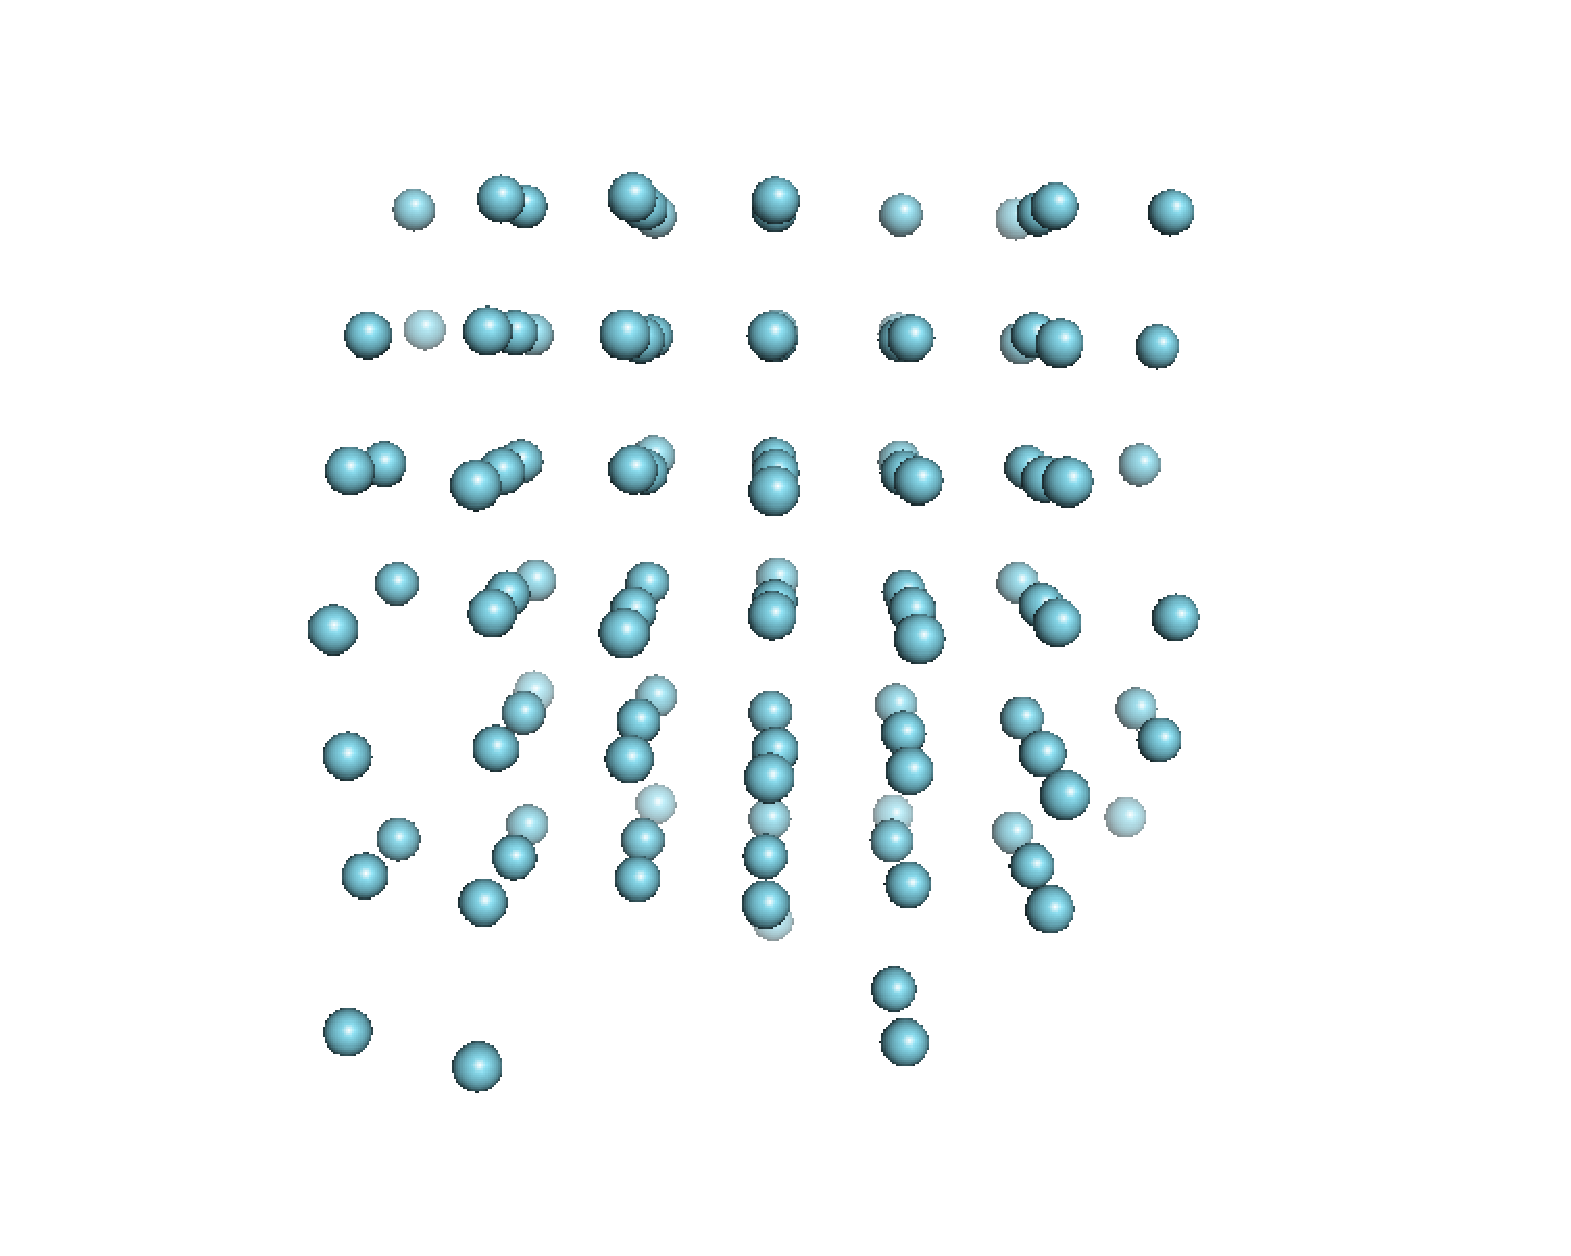
\includegraphics[scale=.25]{ar108scalet4000.pdf}
 \label{fig:ar108scaletemp-4000}
}
\subfigure[Configuraci\'on de Ar al finalizar la simulaci\'on.]
{
 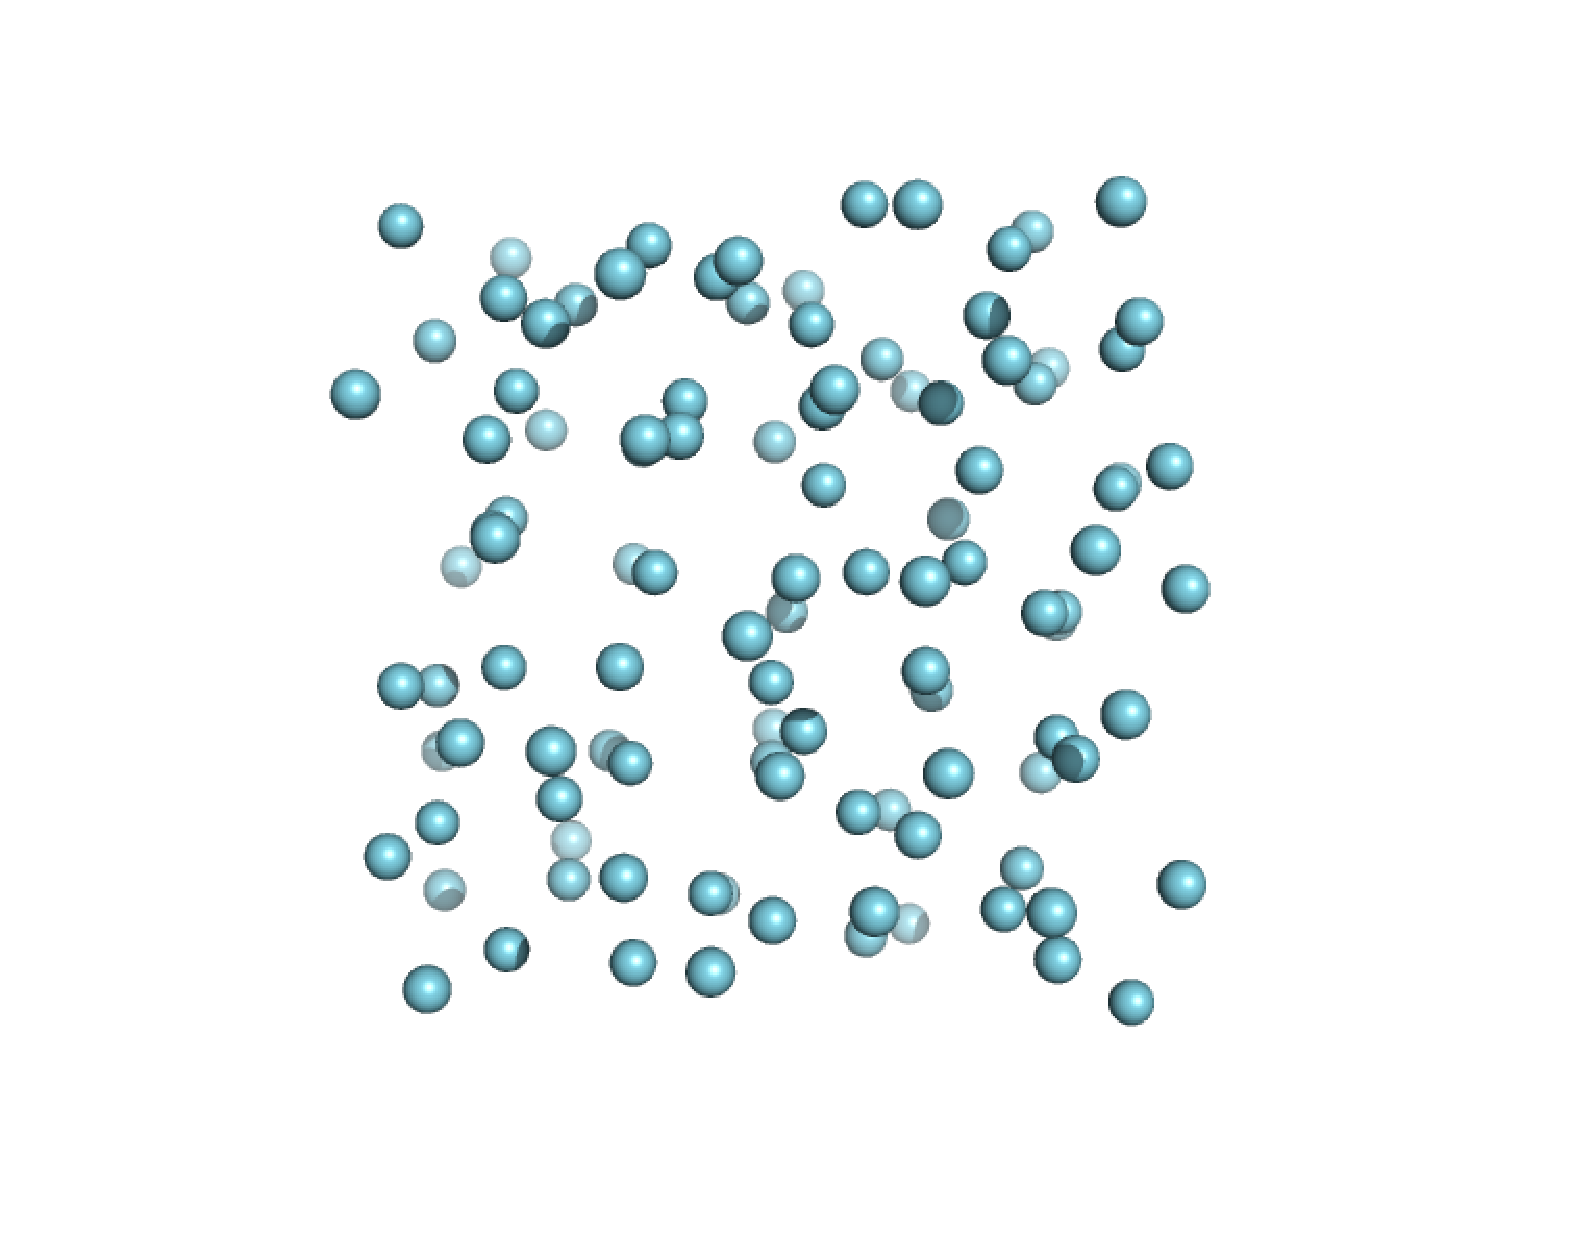
\includegraphics[scale=.25]{ar108scalet15000.pdf}
 \label{fig:ar108scaletemp-15000}
}
\caption{Distintos pasos de una simulaci\'on de din\'amica molecular de 108 \'atomos de Argon.}
\label{fig:ar108scaltemp}
\end{figure}

Adem\'as de este escalamiento de temperatura cl\'asico, \lpmd posee dentro de sus plugins otros termostatos, refierase al cap\'itulo\ref{chap:modulos}

\subsection{Escalamiento de Celda.}

Modificaremos las caracter\'isticas de la celda durante la simulaci\'on, para ello haremos uso del m\'odulo cellscaling, y luego veremos como se modifica la presi\'on del sistema, junto con la temperatura, el ejemplo esta disponible en

\cajatx{http://wwww.gnm.cl/software/lpmd/examples/ar108-scalec.tgz}

De manera similar a la anterior, se carga un modulo que modifica una propiedad de nuestro sistema, para llevarlo a las condiciones deseadas. En el siguiente fichero de control, se ve como se escala una celda.

\begin{multicols}{2}
\setlength{\columnseprule}{.5pt}
\begin{verbatim}
# System file of Ar gas 
# using LPMD
#
###################
#CELL and IN/OUT###
###################
cell crystal a=17.1191 b=17.1191 \
     c=17.1191 alpha=90.0 \
     beta=90.0 gamma=90.0

input module=lpmd file=Ar108.lpmd
output module=xyz file=output.xyz \
     each=20 level=0
###################
#GENERAL###########
###################
prepare replicate 1 1 1
prepare temperature 84
charge Ar 0.0
steps 15000
dumping file=ljargon.dump each=10000
periodic true true true

#Cargamos inmediatamente pressure
#para poder visualizar con monitor

use pressure
enduse

monitor start=0 end=15000 each=10 \
  properties=kinetic-energy, \
  potential-energy,total-energy, \
  temperature,pressure,volume \
  output=monitor.dat
###################
#MODULES DEF#######
###################
use lennardjones as lj_Ar
    sigma 3.41
    epsilon 0.0103408
    cutoff 8.5
enduse

use beeman
    dt 10.0
enduse

use minimumimage
    cutoff 8.5
enduse

use cellscaling as CS
    axis all
    percent 2
    constant true
enduse
###################
#MOD APPLICATION###
###################
potential lj_Ar Ar Ar
integrator beeman
cellmanager minimumimage
apply CS start=5000 end=10000 each=200
\end{verbatim}
\end{multicols}

Podemos ver entonces, como cambia la presi\'on y el volumen durante la simulaci\'on en las figuras~\ref{fig:ar108scalecpres} y~\ref{fig:ar108scalecvol}, con estos datos, uno puede obtener distintos tipos de propiedades mec\'anicas de los materiales en estudio, por ejemplo m\'odulo de \textit{Bulk}.

\begin{figure}[h!]
\centering
\subfigure[Cambio de Presi\'on en el tiempo.]
{
 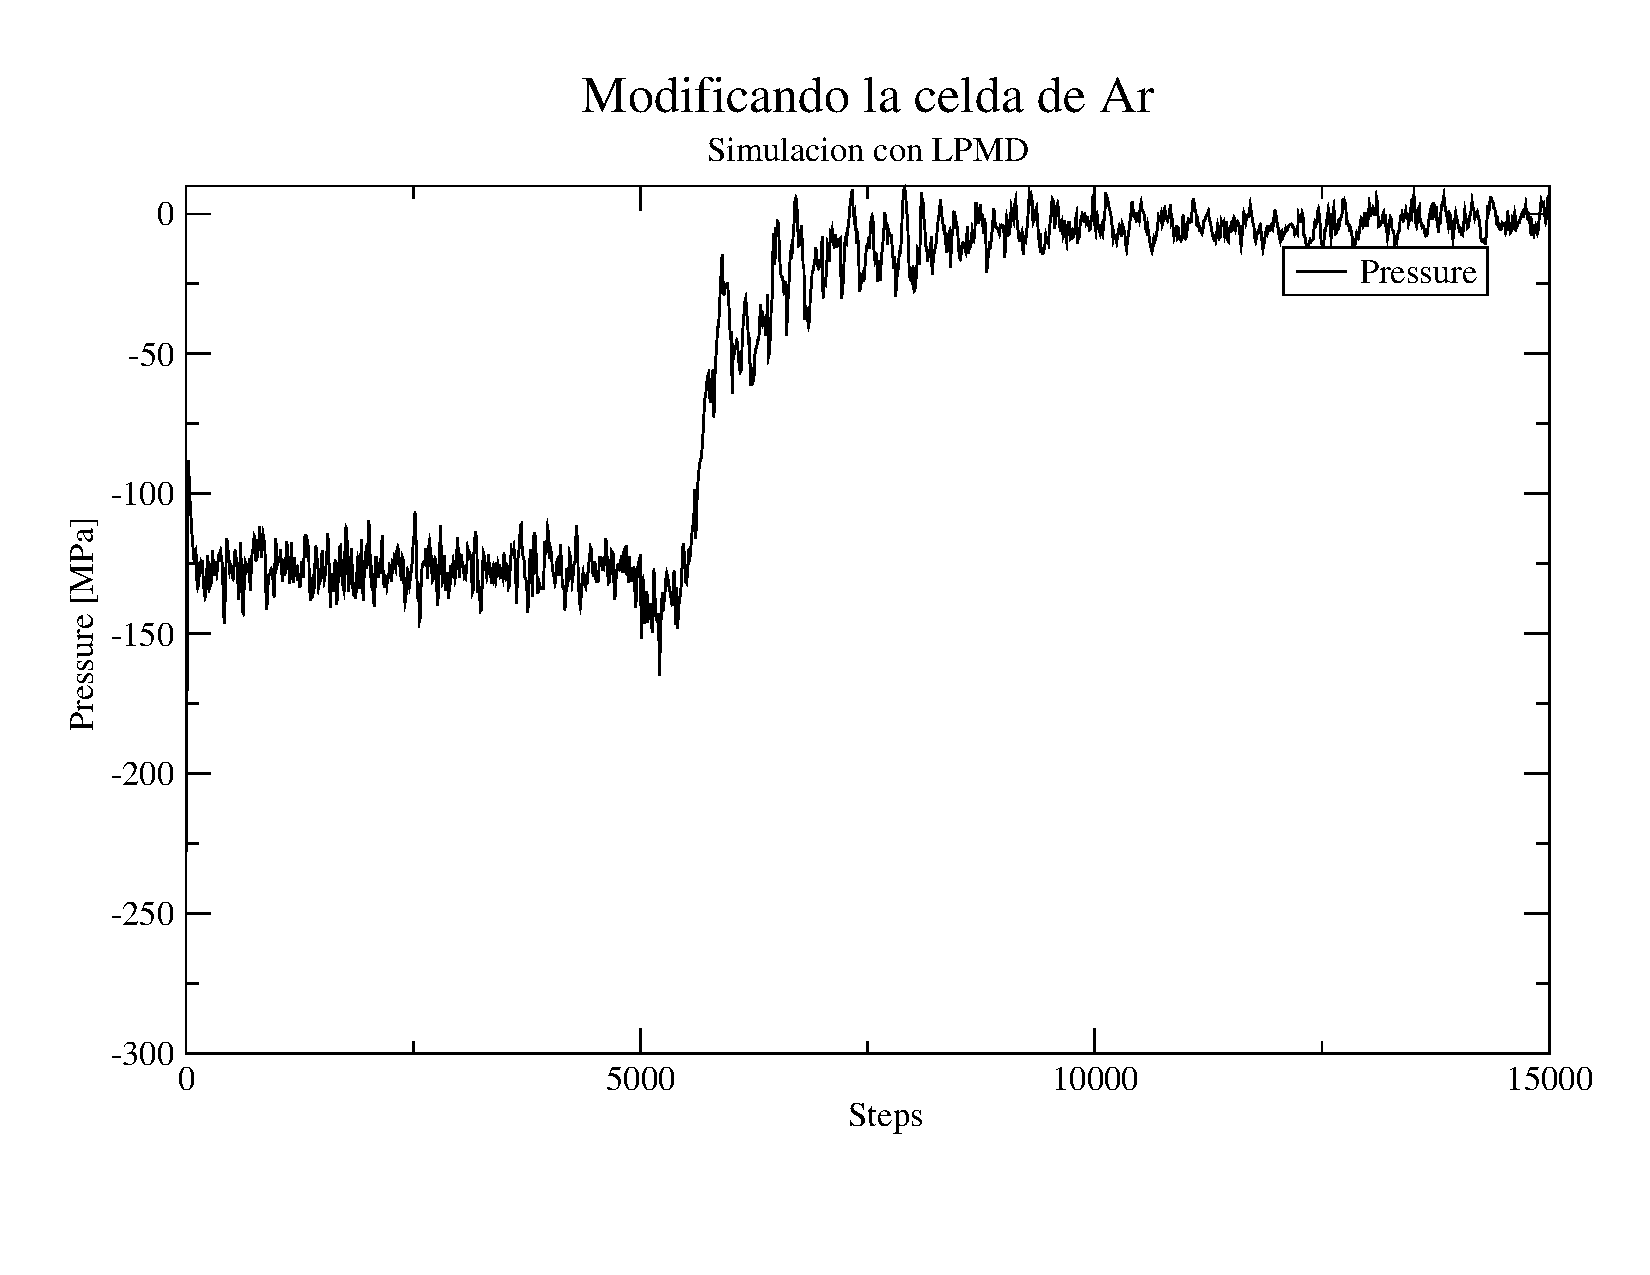
\includegraphics[scale=.25]{ar108scalecpres.pdf}
 \label{fig:ar108scalecpres}
}
\subfigure[Cambio de vol\'umen de la celda durante la simulaci\'on.]
{
 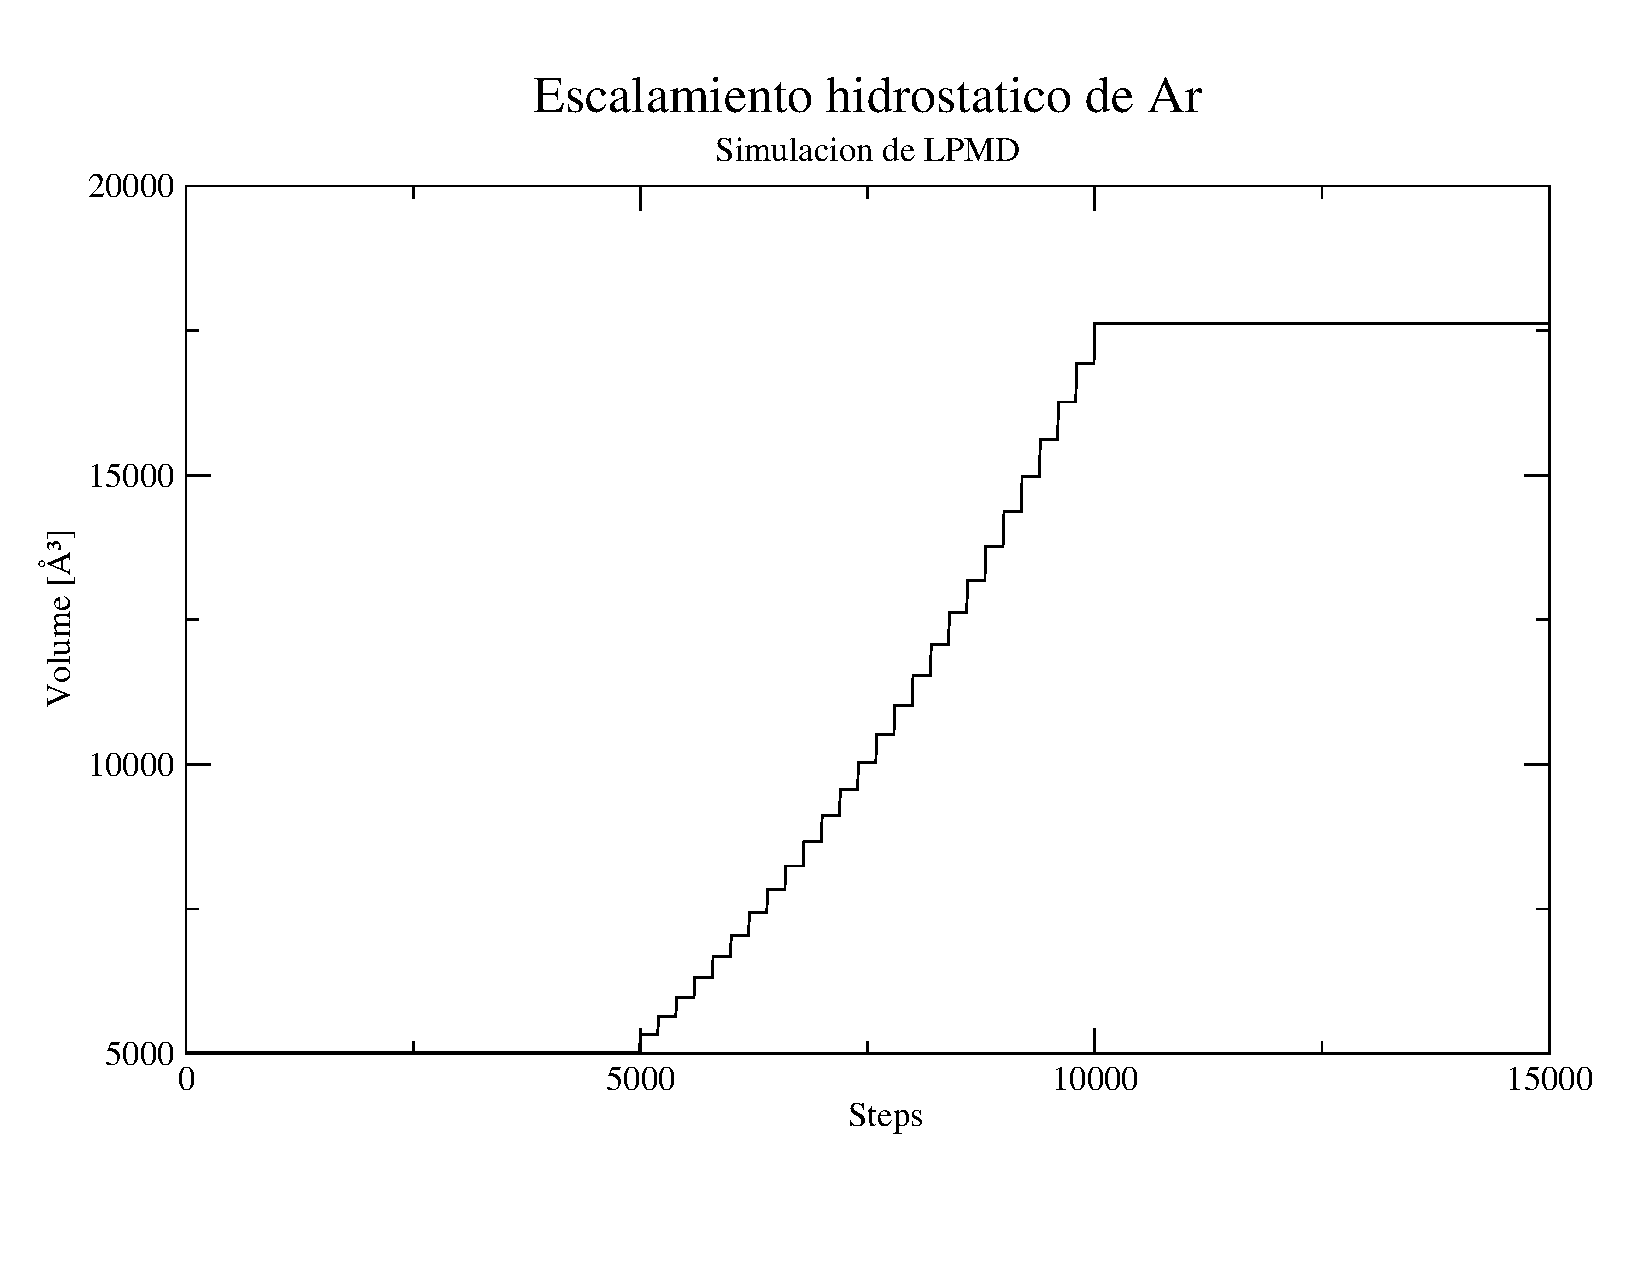
\includegraphics[scale=.25]{ar108scalecvol.pdf}
 \label{fig:ar108scalecvol}
}
\caption{Distintas propiedades del sistema, obtenidas durante la simulaci\'on.}
\label{fig:ar108scalec}
\end{figure}


\subsection{Calculando Propiedades durante la Simulaci\'on.}

A continuaci\'on, realizaremos un procedimiento simple de din\'amica molecular, pero esta vez, con una celda de Oro, sobre la cual calcularemos propiedades, durante la simulaci\'on. En este caso veremos, la \textit{funci\'on radial de distribuci\'on}, \textit{distribuci\'on angular} y \textit{n\'umero de coordinaci\'on}. Adem\'as la informaci\'on en \lpmd puede ser \textbf{subdividida} seg\'un los requerimientos mismos del usuario a la hora de monitorear caracter\'isiticas propias de la celda de simulaci\'on. En este ejemplo, se guarda la informaci\'on de las energ\'ias, y presiones, en dos ficheros \verb|monitor| distintos, para un an\'alisis mucho mas simple. El ejemplo se puede encontrar en:

\cajatx{http://wwww.gnm.cl/software/lpmd/examples/au-prop.tgz}

\begin{multicols}{2}
\setlength{\columnseprule}{.5pt}
\begin{verbatim}
cell crystal a=16.320 b=16.320 \
 c=16.320 alpha=90.0 beta=90.0 \
 gamma=90.0

input module=xyz file=au-input.xyz\
      level=1
output module=xyz \
      file=au-output.xyz each=30 \
      level=1

# Periodicity in x, y, z 
periodic true true true

# Molecular dynamics settings
steps 20000

use pressure
enduse

dumping 5000 au.dump
monitor start=0 end=20000 each=1 \
      properties=kinetic-energy,\
      potential-energy,\
      total-energy,temperature \
      output=monitor-cell.out
monitor start=0 end=20000 each=1 \
      properties=virial-pressure,\
      kinetic-pressure,pressure,\
      volume,sxx,syy,szz \
      output=monitor-pres.out

# Using LSC parameters for gold
use suttonchen as sc
    e 0.013
    n 10
    a 4.08
    m 8
    c 34.408
    cutoff 4
enduse

use velocityverlet
    dt 1.0
enduse

use linkedcell
	nx 2
	ny 2
	nz 2
	cutoff 8
enduse

use gdr
 rcut 10.0
 bins 200
 output gdr.dat
 average true
enduse

use angdist
 bins 200
 atoms 1 Au
 rcut Au Au 3.4
 output angdist.dat
 average true
enduse

use cordnumfunc
 bins 200
 atoms 1 Au
 rcut 10
 output cordnumfunc.dat
 average true
enduse

potential sc Au Au
cellmanager linkedcell
integrator velocityverlet
property gdr start=10000 \
         end=15000 each=50
property angdist start=10000\
         end=15000 each=50
property cordnumfunc start=10000\
         end=15000 each=50
\end{verbatim}
\end{multicols}

Las propiedades calculadas se pueden observar en las figuras ~\ref{fig:augdr}, ~\ref{fig:aunang} y ~\ref{fig:aucnf}.

\begin{figure}[h!b]
\centering
\subfigure[Funci\'on $g(r)$ para celda de Au.]
{
 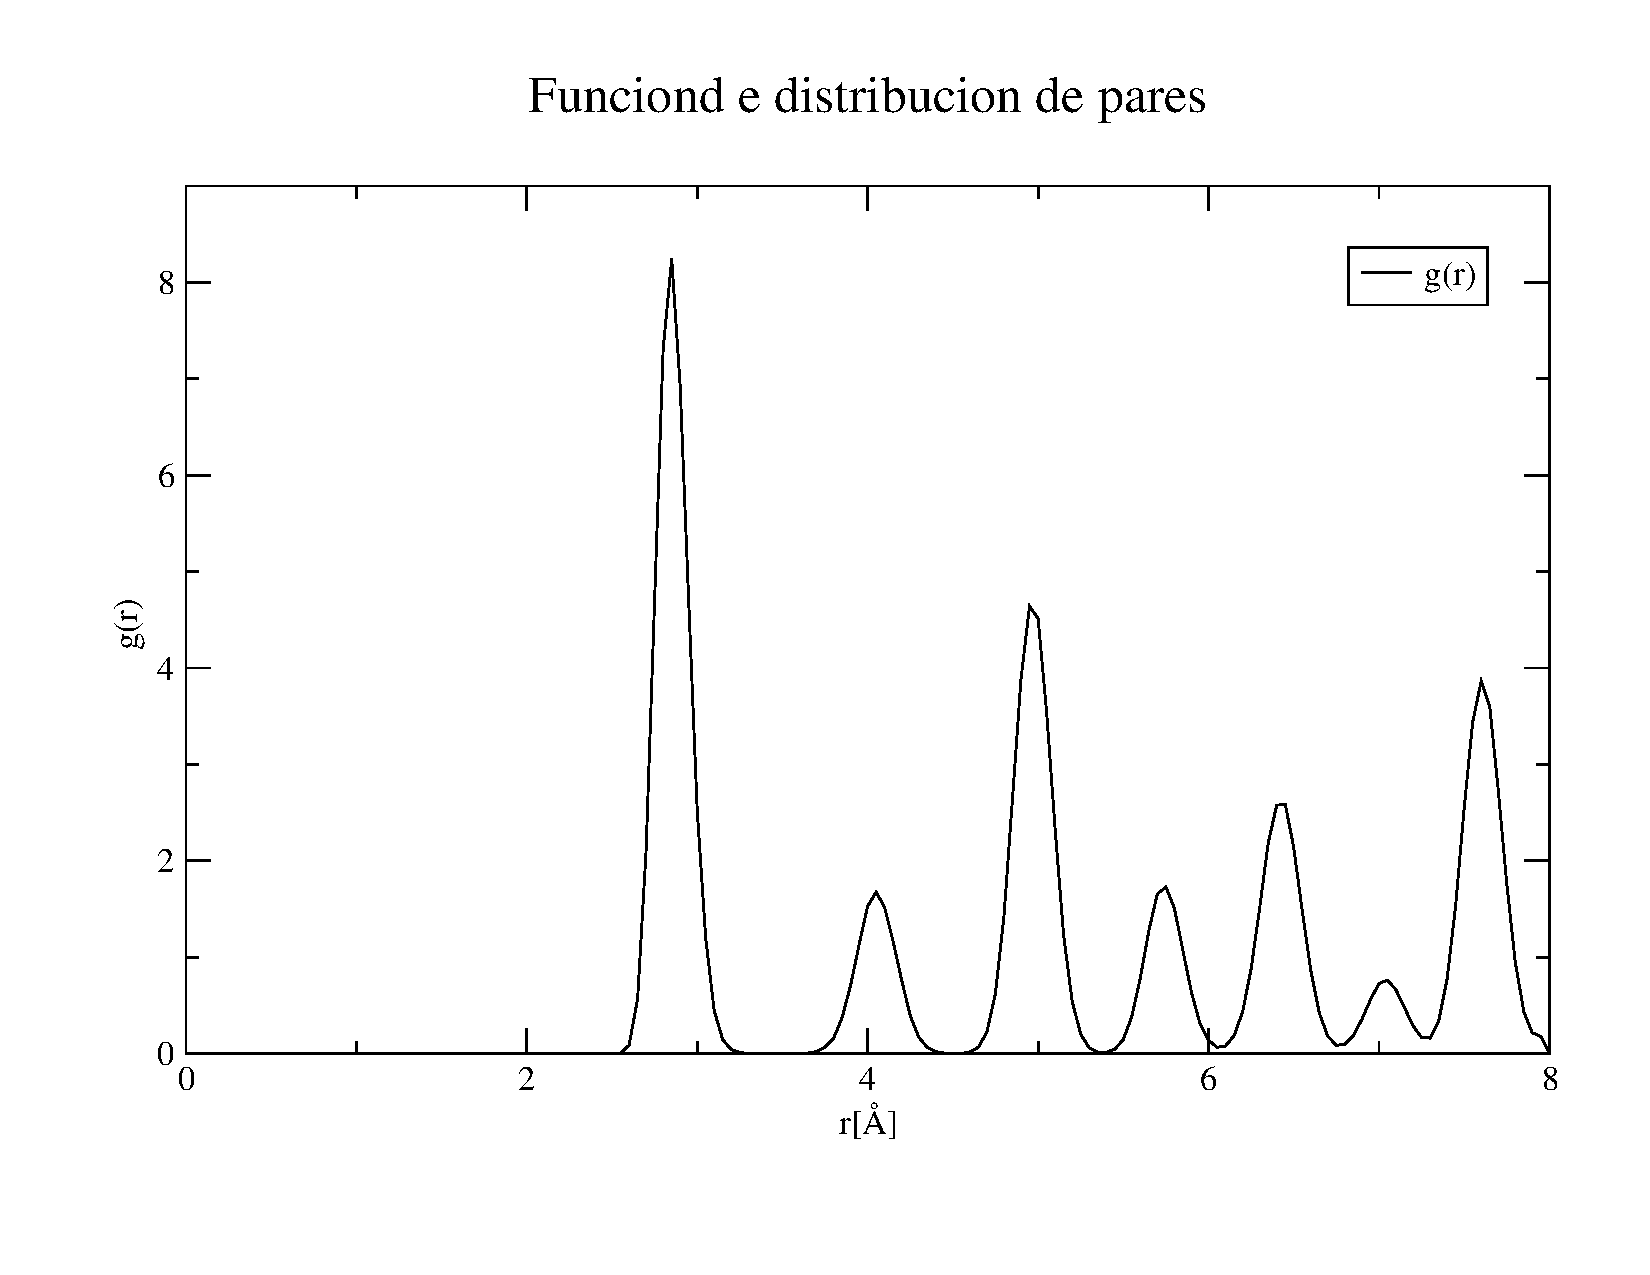
\includegraphics[scale=.25]{augdr.pdf}
 \label{fig:augdr}
}
\subfigure[Funci\'on de distribuci\'on angular.]
{
 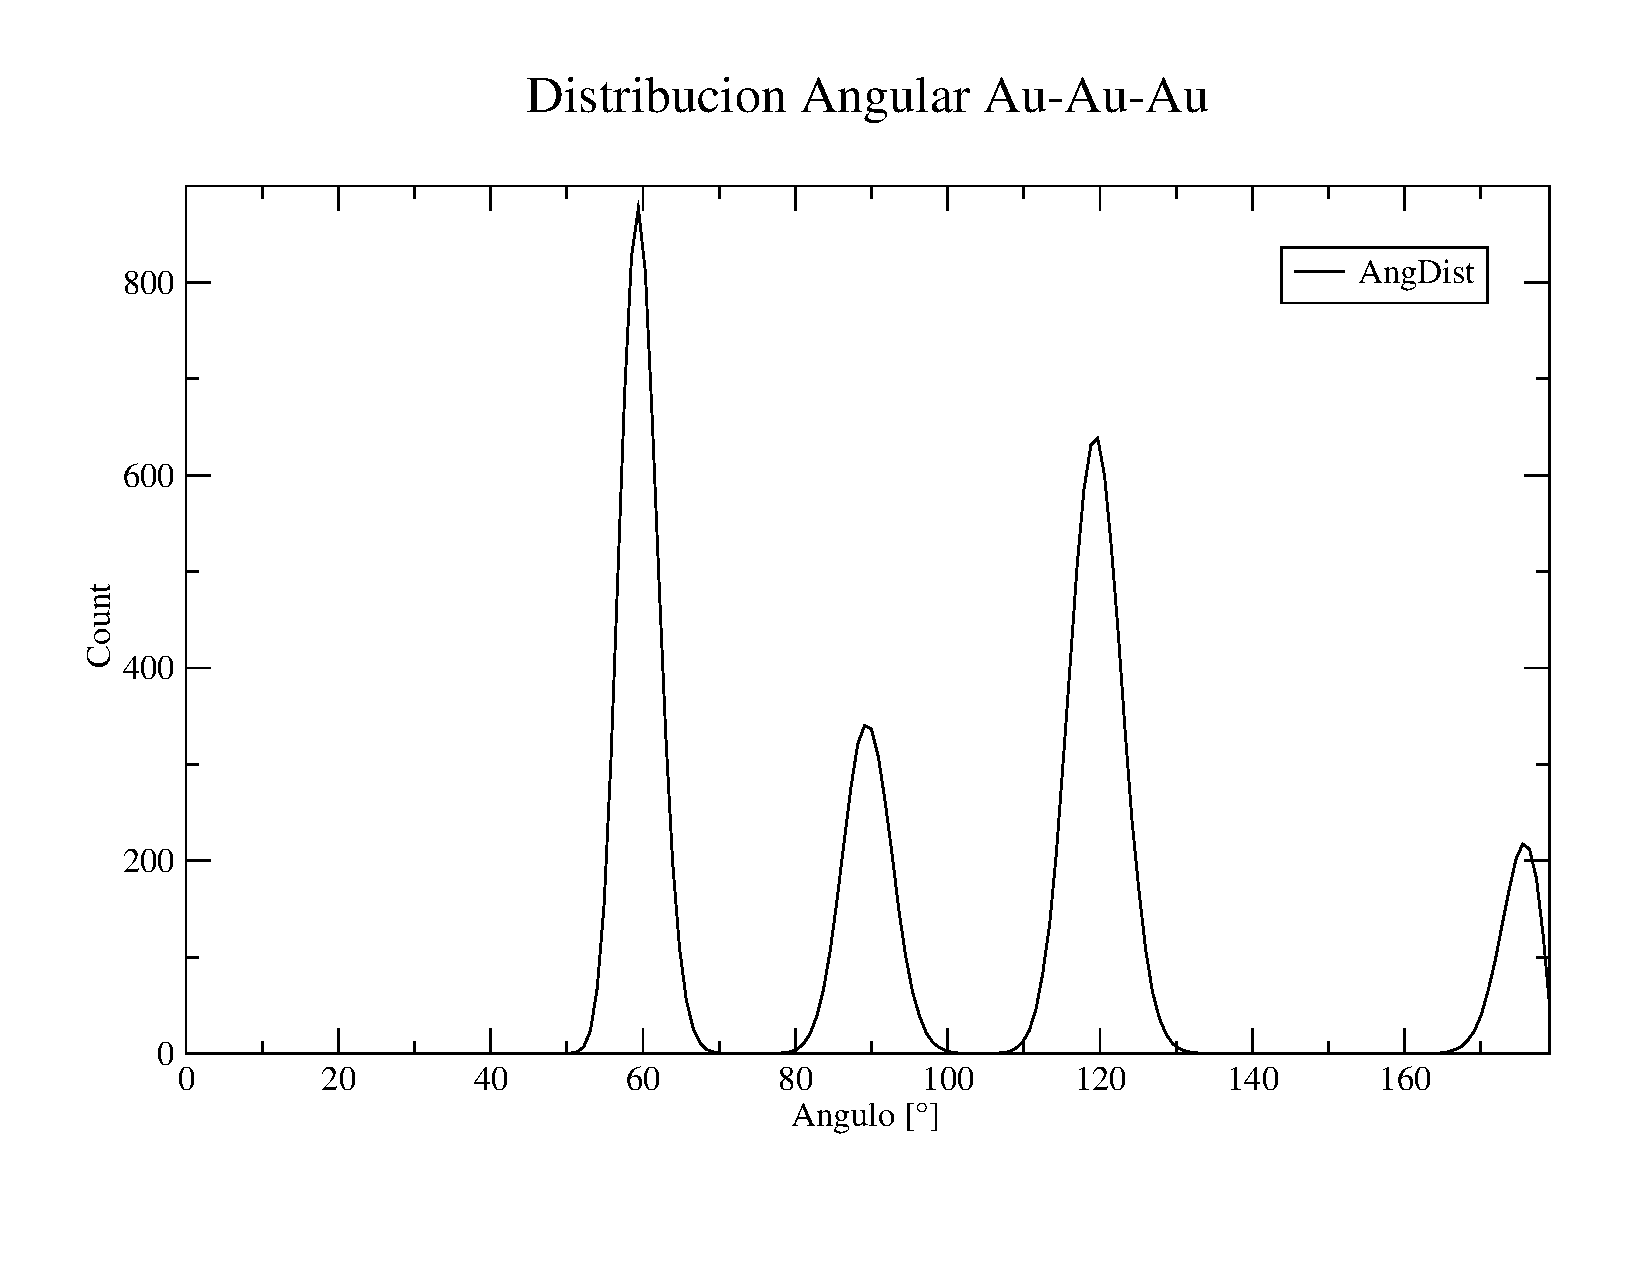
\includegraphics[scale=.25]{aunang.pdf}
 \label{fig:aunang}
}
\subfigure[N\'umero de coordinaci\'on.]
{
 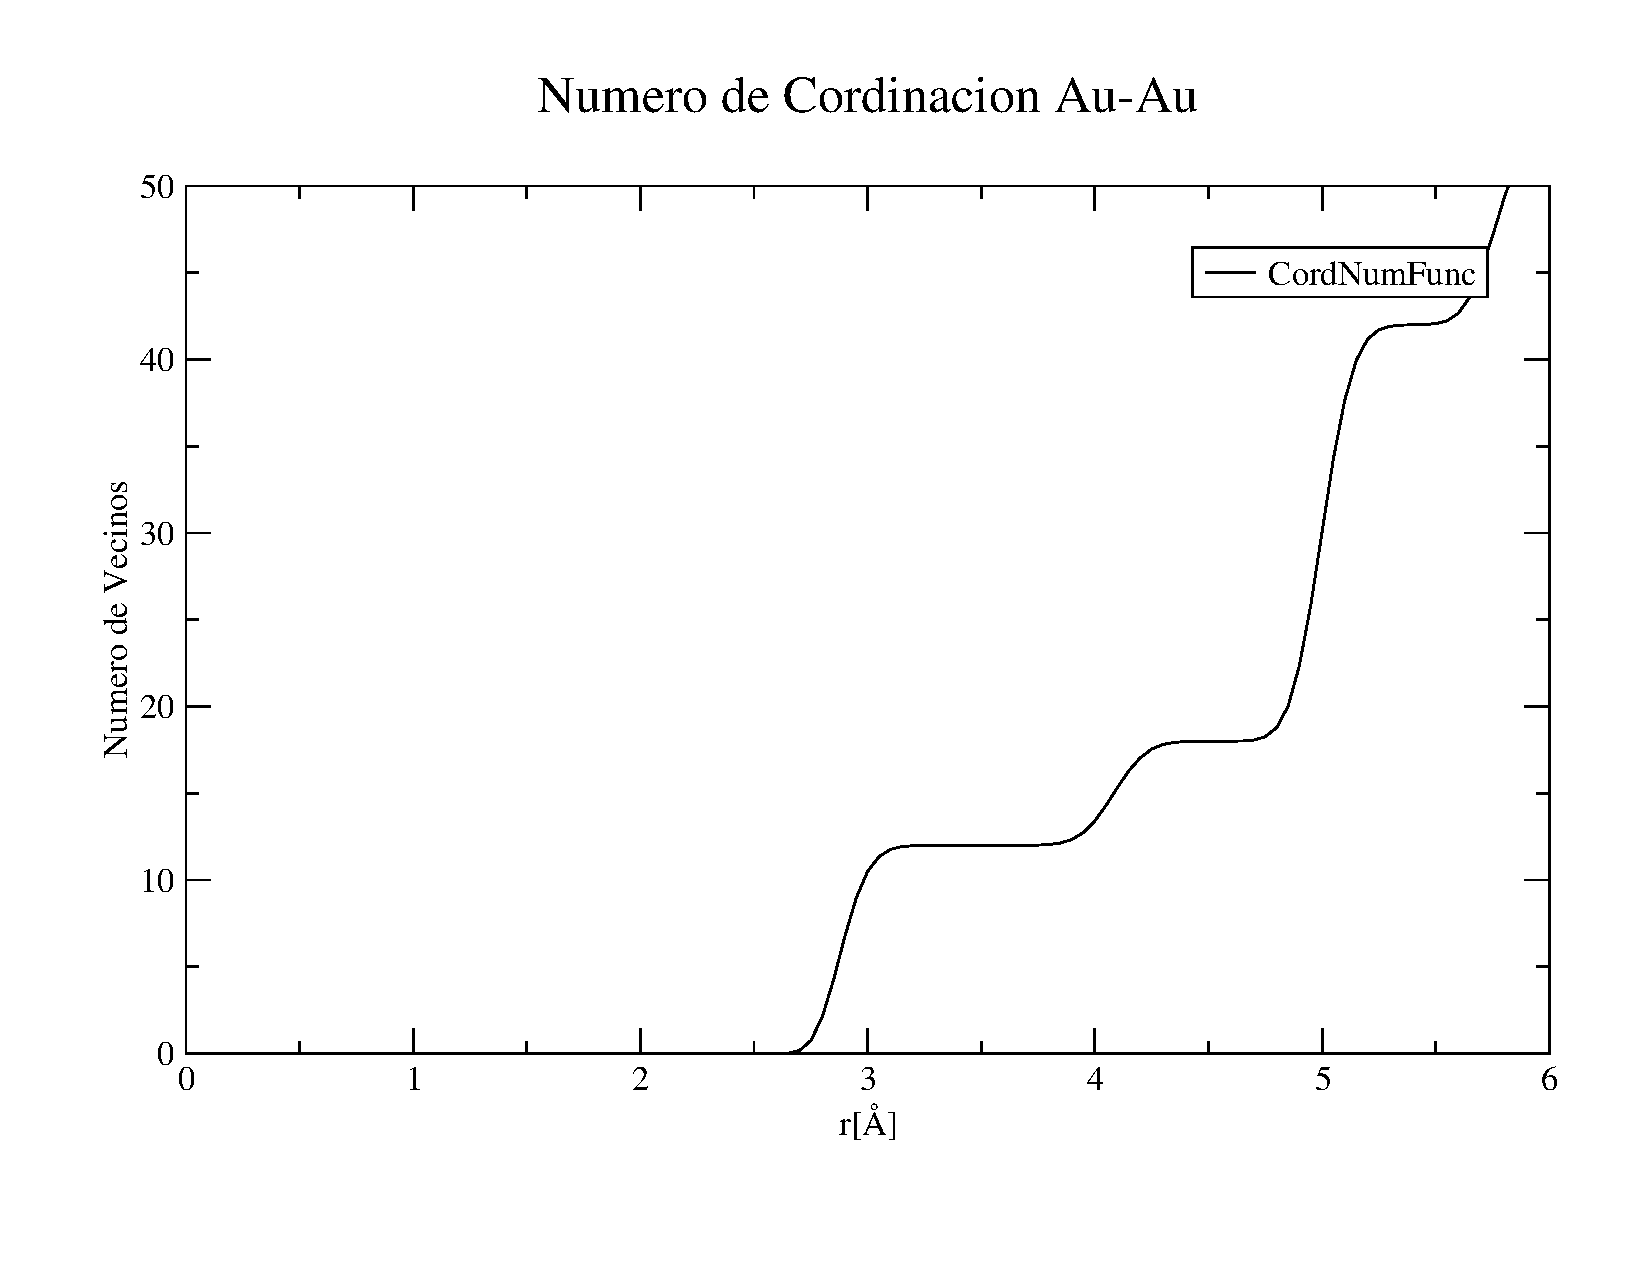
\includegraphics[scale=.25]{aucnf.pdf}
 \label{fig:aucnf}
}
\caption{Propiedades calculadas durante una simulaci\'on de una celda de Au.}
\label{fig:auprop}
\end{figure}

\subsection{Multiples corridas con bash.}

Haremos a continuaci\'on un peque\~no estudio de un gas de Ar a distintas temperaturas, para ello nos respaldaremos de los flags del comando \lpmd para poder modificar variables a partir de un fichero de control, relizaremos un estudio de la \textit{funci\'on de distribuci\'on de pares} para argon bajo distintas temperaturas.

Las temperaturas iniciales que se utilizar\'an son de 5, 100 y 200 Kelvin, estas tres simulaciones podemos realizarlas a partir de un s\'olo fichero de control, como el que se ve a contianuaci\'on:

\begin{multicols}{2}
\setlength{\columnseprule}{.5pt}
\begin{verbatim}
# System file of Ar gas 
# using LPMD
#
###################
#CELL and IN/OUT###
###################
cell crystal a=17.1191 b=17.1191 \
     c=17.1191 alpha=90.0 \
     beta=90.0 gamma=90.0

input module=lpmd file=Ar108.lpmd
output module=xyz \
     file=output-$(INITIALTEMP).xyz \
     each=20 level=0
###################
#GENERAL###########
###################
prepare replicate 1 1 1
prepare temperature $(INITIALTEMP)
charge Ar 0.0
steps 15000
dumping file=ljargon.dump each=10000
periodic true true true

#Cargamos inmediatamente pressure
#para poder visualizar con monitor

use pressure
enduse

monitor start=0 end=15000 each=10 \
  properties=kinetic-energy, \
  potential-energy,total-energy, \
  temperature,pressure,volume \
  output=monitor-$(INITIALTEMP).dat
###################
#MODULES DEF#######
###################
use lennardjones as lj_Ar
    sigma 3.41
    epsilon 0.0103408
    cutoff 8.5
enduse

use beeman
    dt 10.0
enduse

use minimumimage
    cutoff 8.5
enduse

use gdr
 bins 200
 rcut 20
 output gdr-$(INITIALTEMP).dat
 average true
enduse
###################
#MOD APPLICATION###
###################
potential lj_Ar Ar Ar
integrator beeman
cellmanager minimumimage
property gdr start=10000 \\
   end=15000 each=30
\end{verbatim}
\end{multicols}

Esta configuraci\'on generara archivos \verb|monitor|, \verb|output| y \verb|gdr| de forma independiente para cada una de las temperaturas, para correrlo basta con :

\begin{center}
 \texttt{for i in 5 100 200 ; \\do lpmd -o TEMP=\$i opcion-o.control > simulacion-\$i.info ; done}
\end{center}

Los resultados de la funcion radial de distribuci\'on de pares, pueden observarse en las figuras ~\ref{fig:opogdr5}, ~\ref{fig:opogdr100} y ~\ref{fig:opogdr200}, donde se ve claramente que la condici\'on de temperatura inicial es un factor importante en el desarrollo de la din\'amica molecular ya que son las condiciones iniciales con las que comienza el sistema su evoluci\'on.

\begin{figure}[h!]
\centering
\subfigure[Funci\'on $g(r)$ para 5K.]
{
 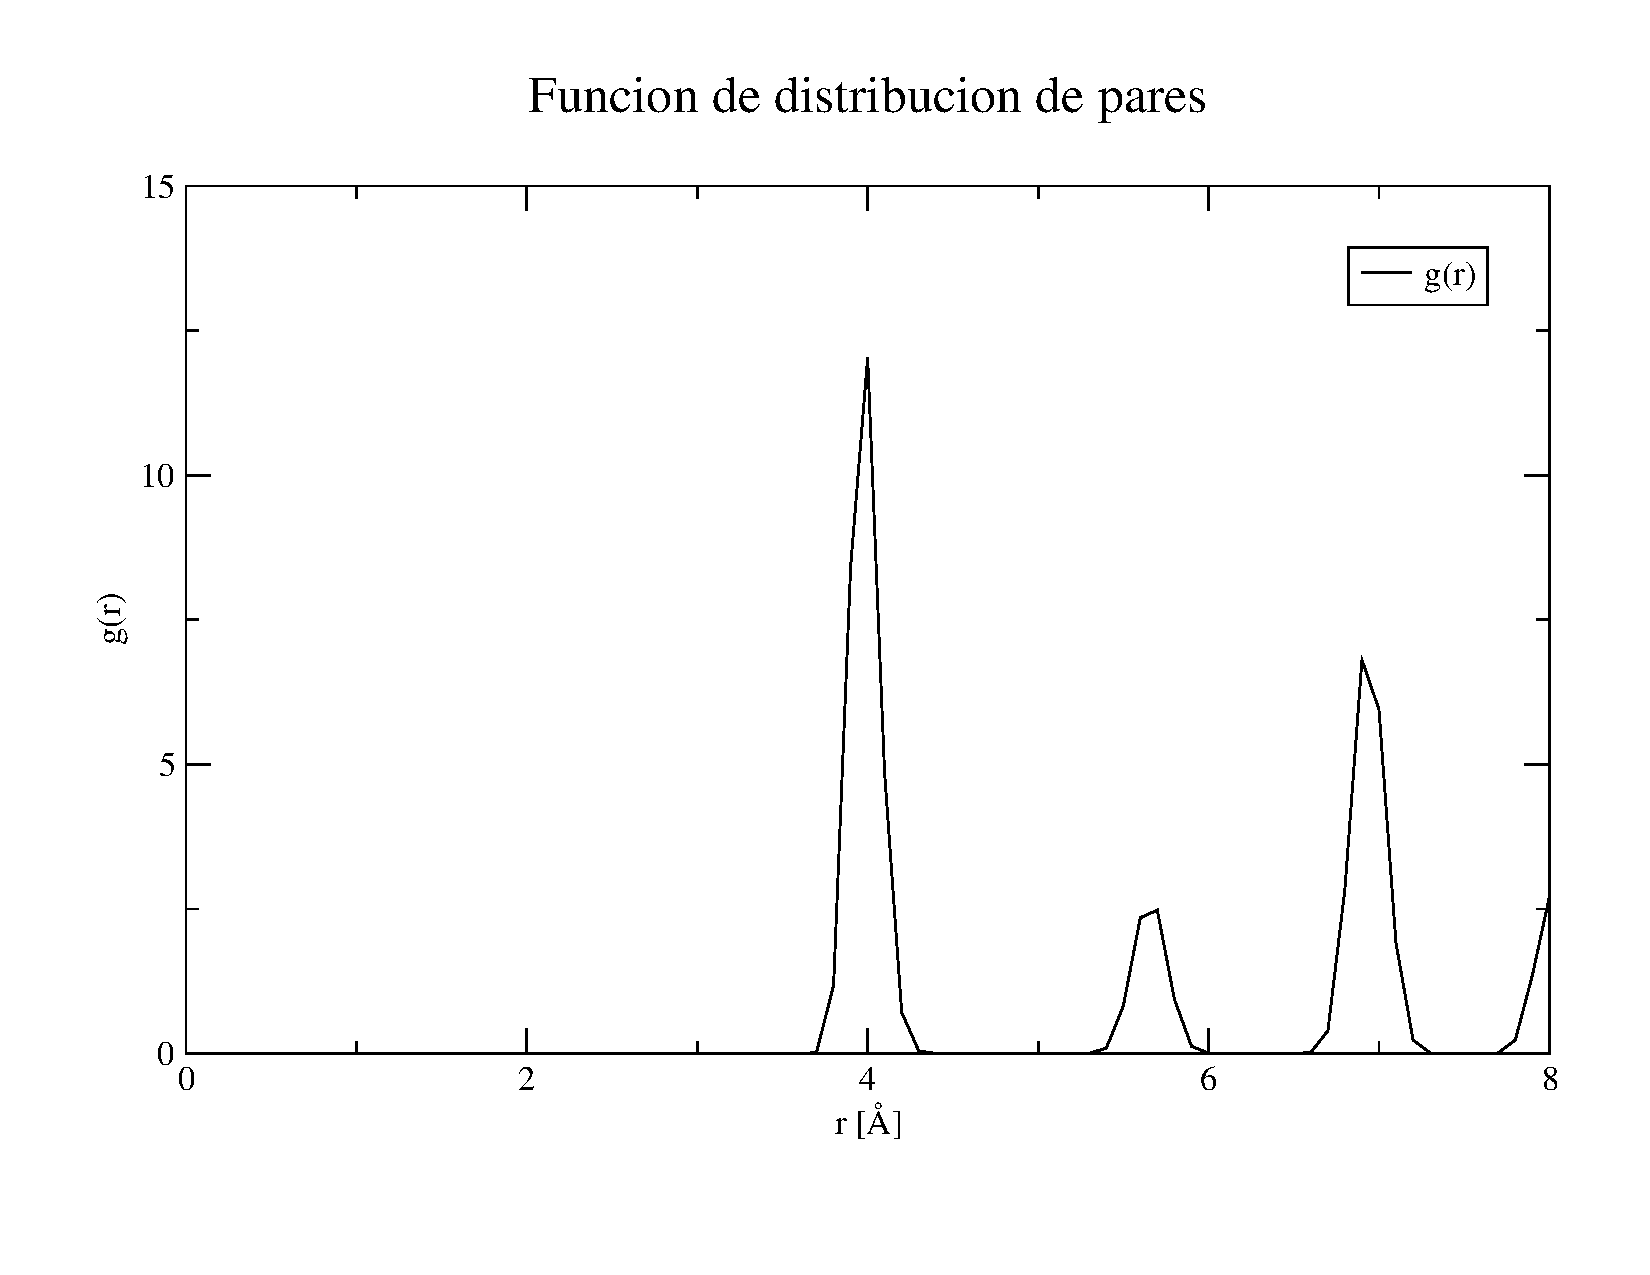
\includegraphics[scale=.25]{opogdr5.pdf}
 \label{fig:opogdr5}
}
\subfigure[Funci\'on $g(r)$ para 100K.]
{
 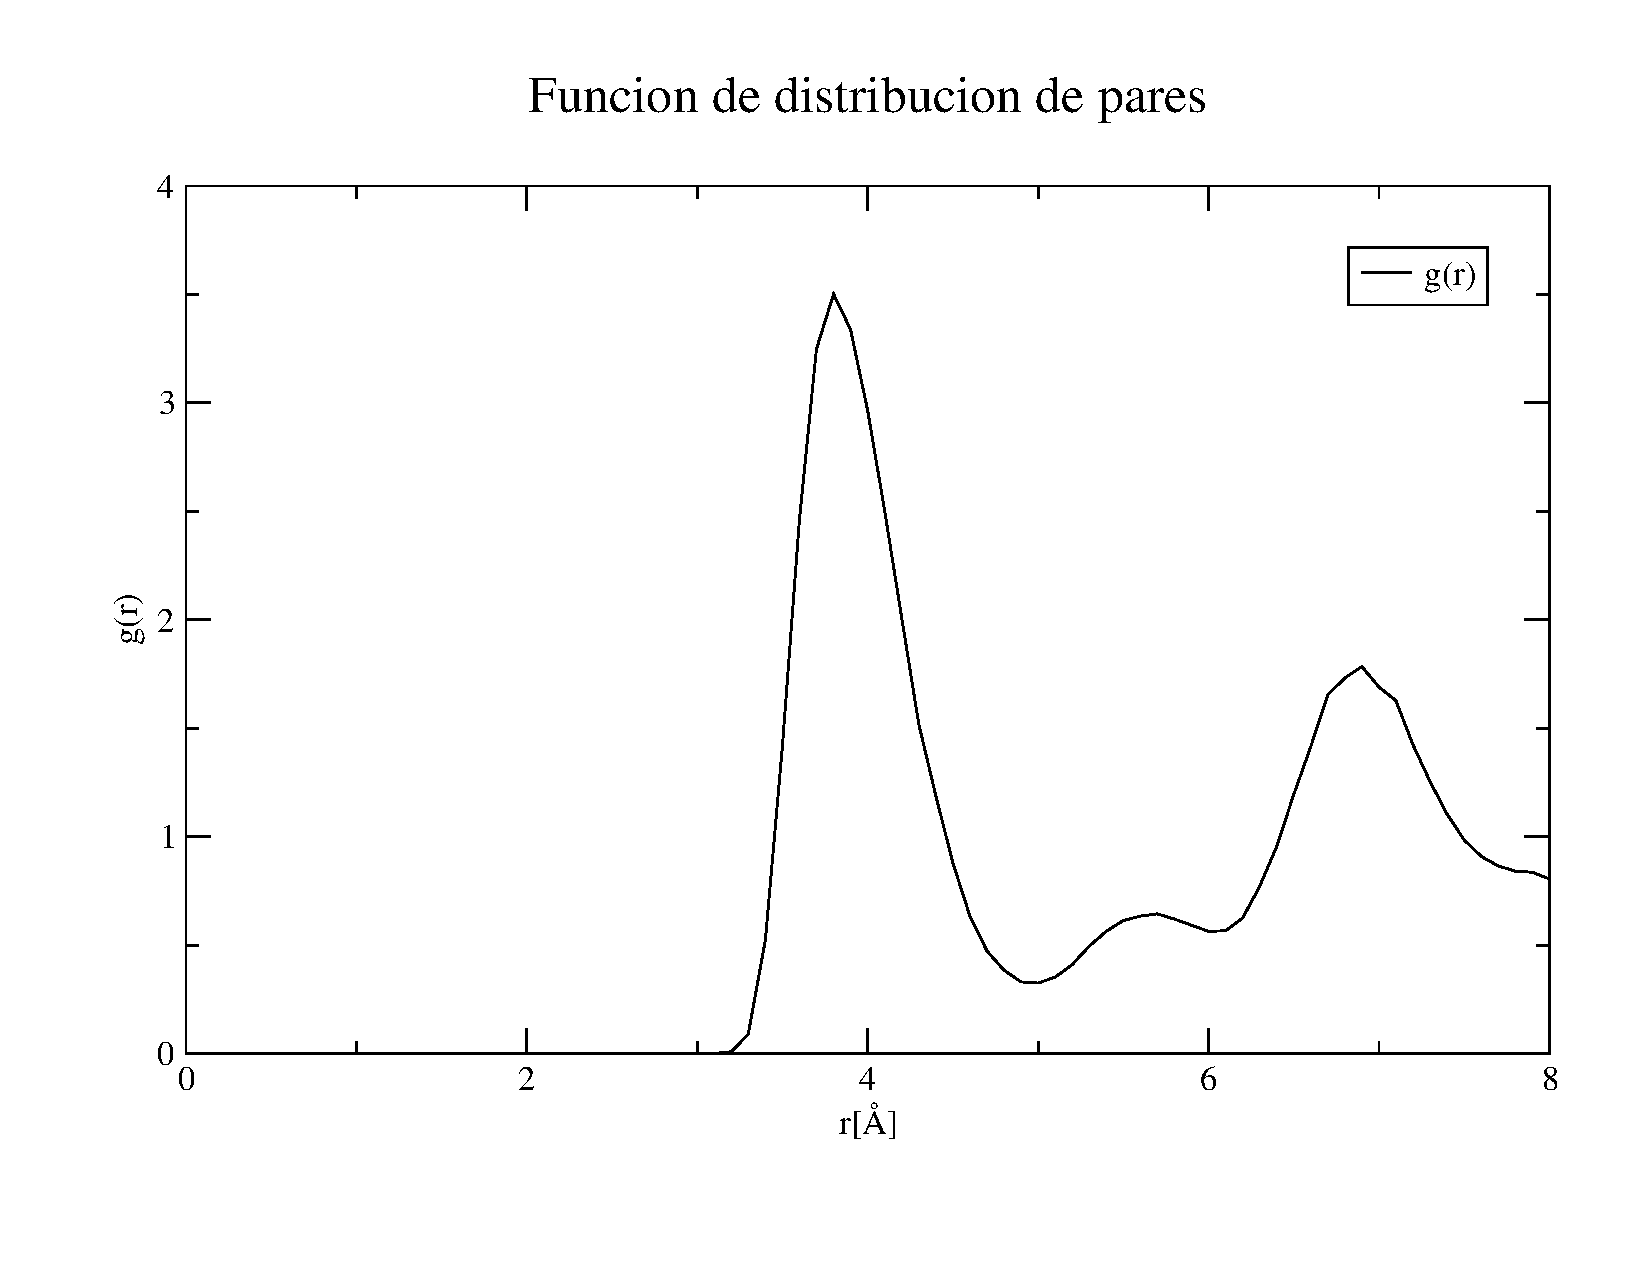
\includegraphics[scale=.25]{opogdr100.pdf}
 \label{fig:opogdr100}
}
\subfigure[Funci\'on $g(r)$ para 200K.]
{
 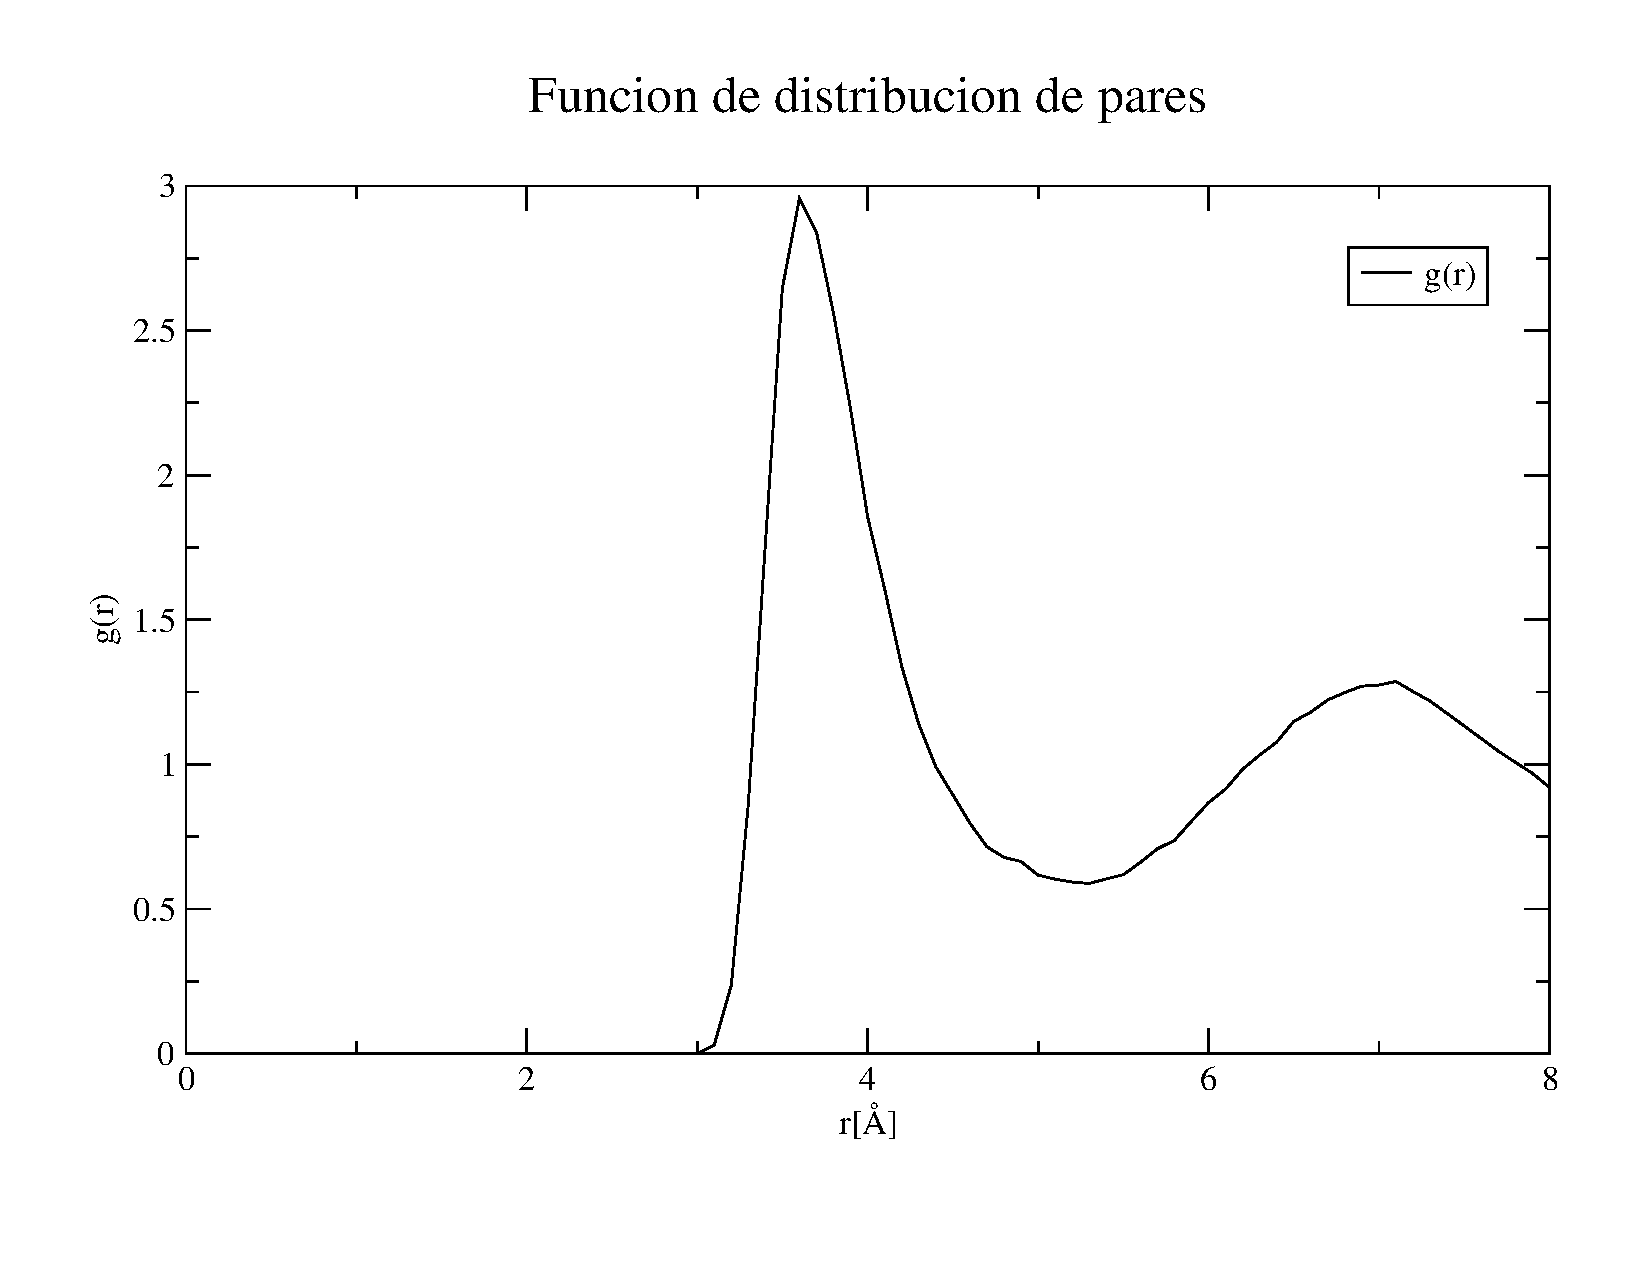
\includegraphics[scale=.25]{opogdr200.pdf}
 \label{fig:opogdr200}
}
\caption{Funci\'on $g(r)$ para distintas temperaturas iniciales del sistema.}
\label{fig:opogdr}
\end{figure}


\subsection{Generando ficheros pov para crear pel\'iculas.}

Fue uno de los primeros \textit{approach} a lo que a m\'odulos de visualizaci\'on se refiere, su intenci\'on es generar, a partir de la simulaci\'on, un set de ficheros \verb|pov| para un posterior renderizado y creaci\'on de peliculas, animaciones o simplemente imagnes de alta calidad. El ejemplo puede descargarse en:

\cajatx{http://wwww.gnm.cl/software/lpmd/examples/arpovmul.tgz}

Veamos a continuacion el c\'odigo utilizado para la simulaci\'on:

\begin{multicols}{2}
\setlength{\columnseprule}{.5pt}
\begin{verbatim}
# System file of Ar gas 
# using LPMD
#
###################
#CELL and IN/OUT###
###################
cell crystal a=17.1191 b=17.1191 \
   c=17.1191 alpha=90.0 beta=90.0 \
   gamma=90.0

input module=lpmd file=Ar108.lpmd
output module=xyz file=output.xyz \
   each=20 level=0
###################
#GENERAL###########
###################
prepare replicate 2 2 2
prepare temperature 84
charge Ar 0.0
steps 10
dumping file=ljargon.dump each=5
periodic true true true

#Cargamos inmediatamente pressure
#para poder visualizar con monitor

use pressure
enduse

monitor start=0 end=5000 each=10 \
  properties=kinetic-energy, \
  potential-energy,total-energy, \
  pressure,volume output=monitor.dat
###################
#MODULES DEF#######
###################
use lennardjones as lj_Ar
    sigma 3.41
    epsilon 0.0103408
    cutoff 8.5
enduse

use beeman
    dt 10.0
enduse

use minimumimage
    cutoff 8.5
enduse

use povray
    header shoot-
    direct movie
    text "Modelacion de Ar" <dl> \
      <green> [3] ()
    text " Step = % " <uc> <red> [3] \
      (Step)
    rotate <0,45,0>
    background <1,1,1>
enduse

###################
#MOD APPLICATION###
###################
potential lj_Ar Ar Ar
integrator beeman
cellmanager minimumimage
visualize povray start=0 \
   end=10 each=1
\end{verbatim}
\end{multicols}

%El resultado de la simulaci\'on es la generaci\'on de ficheros \verb|pov| que se encuentran dentro del directorio \verb|movie|, es importante destacar que la conversion de estos ficheros \verb|pov| en im\'agenes de alta calidad, puede llevarse a cabo con \verb|povray|, un software libre de renderizado de imagenes. Un resultado de la conversi\'on de una im\'agen pude verse en la figura~\ref{fig:povrayex}

\begin{figure*}[h!]
\begin{minipage}{8cm}
 El resultado de la simulaci\'on es la generaci\'on de ficheros \verb|pov| que se encuentran dentro del directorio \verb|movie|, es importante destacar que la conversion de estos ficheros \verb|pov| en im\'agenes de alta calidad, puede llevarse a cabo con \verb|povray|, un software libre de renderizado de imagenes. Un resultado de la conversi\'on de una im\'agen pude verse en la figura~\ref{fig:povrayex}
\end{minipage}
\hfill
\begin{minipage}{7cm}
\centering
 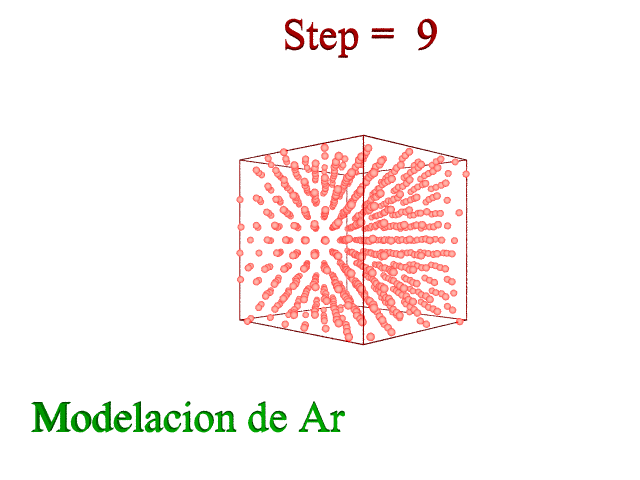
\includegraphics[scale=.3]{shoot-pov.png}
\caption{Im\'agen resultante de los ficheros \texttt{pov} generados en la simulaci\'on.}
\label{fig:povrayex}
\end{minipage}
\end{figure*}

% \subsection{Cambiando el integrador durante la simulaci\'on.}
% 
% Una caracter\'istica de \lpmd es poder cambiar el integrador, durante la simulaci\'on, esto es utilizado en un ejemplo a continuaci\'on que puede descagar en:
% 
% \cajatx{http://wwww.gnm.cl/software/lpmd/examples/int-change.tgz}
% 
% \subsection{Calculo de Modulo de Bulk}
% 
% En este ejemplo, se calcula el m\'odulo de Bulk para Au modificando el tama\~no de la celda de forma hidrostatica durante la simulaci\'on, para as\'i obtener directamente las presiones.

%%%%%%%%%%%%%%%%%%%%%%%%%%%%%%%%%%%%%%%%%%%%%%%%%%%%%%%%%%%%%%%%%
%%%%%%%%%%%%%%%%%%%%%%%%%%%%%%%%%%%%%%%%%%%%%%%%%%%%%%%%%%%%%%%%%
\section{Ejemplos LPMD-ANALYZER}

La funci\'on principal de \textbf{lpmd-analyzer} es poder cargar configuraciones de distinto tipo, tales como \verb|xyz| o \verb|lpmd| para poder obtener an\'alisis de estas configuraciones.

Para los ejemplos de \textbf{lpmd-analyzer} utilizaremos un fichero de tipo \verb|xyz| proveniente de una simulaci\'on de din\'amica molecular hecha con \textbf{moldy} de di\'oxido de germanio, o germania, como se ve en la figura~\ref{fig:geo2-1}.

\cajafi{geo2-1.pdf}{Una de las configuraciones de GeO$_2$ bajo condicion ambiente, del total de configuraciones obtendremos distintas propiedades utilizando \textbf{lpmd-analyzer}.}{geo2-1}

\subsection{Calculando funci\'on radial de distribuci\'on.}

Tomamos un fichero \verb|xyz| y obtenemos la funci\'on de distribuci\'on radial del sistema, este fichero consta de 50 configuraciones, para obtener gdr utilizamos un fichero de \verb|control|, pero a diferencia de los ficheros de control de \lpmd, este fichero cuenta solo con lo necesario para evaluar una propiedad, como se ve a continuaci\'on:

\begin{multicols}{2}
\setlength{\columnseprule}{.5pt}
\begin{verbatim}
#Fichero que calcula g(r)
#para un fichero xyz con 100 
#configuraciones

cell cubic a=20.7
input module=xyz file=final20p8.xyz \
      inside=true

use linkedcell
   nx 2
   ny 2
   nz 2
   cutoff 10
enduse

use gdr as pgdr
   bins 200
   rcut 15
   output gdr.dat
   average true
enduse

cellmanager linkedcell
property pgdr start=1 end=100 each=1
\end{verbatim}
\end{multicols}

De esta forma calculamos la funci\'on radial de distribuci\'on ejecutando \verb|lpmd-analyzer gdr.control| lo que guardara la informaci\'on de la $g(r)$ en el fichero \verb|gdr.dat| promediando cada uno de los c\'alculos realizados. l resultado final del calculo de $g(r)$ se puede ver en la figura~\ref{fig:exagdr}.

\cajafi{gdr.pdf}{Funci\'on radial de distribuci\'ond e pares, note que \texttt{lpmd-analyzer}, autom\'aticamente calcula para cada una de las especies at\'omicas de la muestra y para el total.}{exagdr}

\subsection{Desplazamiento Cuadr\'atico Medio.}

Calcularemos ahora el desplazamiento cuadr\'atico medio (\verb|msd|) de nuestra muestra, utilizando el m\'odulo \verb|msd|. El archivo de control, se muestra a continuaci\'on:

\begin{multicols}{2}
\setlength{\columnseprule}{.5pt}
\begin{verbatim}
#Fichero que calcula g(r)
#para un fichero xyz con 100 
#configuraciones

cell cubic a=20.7
input module=xyz file=final20p8.xyz \
      inside=true

use linkedcell
   nx 2
   ny 2
   nz 2
   cutoff 10
enduse

use msd as pmsd
   output msd.dat
enduse

cellmanager linkedcell
property pmsd start=1 end=100 each=1
\end{verbatim}
\end{multicols}

\cajafi{msd.pdf}{Desplazamiento cuadr\'atico medio (\texttt{msd}) calculado con \texttt{lpmd-analyzer}.}{examsd}

Note que la actual versi\'on del plugin \verb|msd|, no da la informaci\'on de especie por cada columna entregada, como se ve en la figura~\ref{fig:examsd}, por ahora el an\'alisis debe realizarlo usted cada vez. Se corregir\'a en la pr\'oxima versi\'on de \verb|msd|.

\subsection{Calculando distribucion angular.}

Para el c\'alculo de la distribuci\'on angular, utilizaremos las muestras de GeO$_2$ bajo condicion ambiente que fueron tomadas luego de la simulaci\'on. El fichero de control es de la forma:

\begin{multicols}{2}
\setlength{\columnseprule}{.5pt}
\begin{verbatim}
#Calcula distribucion angular
#para un fichero xyz con 100 
#configuraciones

cell cubic a=20.7

input module=xyz file=final20p8.xyz /
      inside=true

use linkedcell
   nx 2
   ny 2
   nz 2
   cutoff 10
enduse

use angdist as ang
   bins 200
   atoms 2 Ge O
   rcut Ge Ge 3.6
   rcut Ge O  1.9
   rcut O  O  3.2
   output ang.dat
   average true
enduse

cellmanager linkedcell
property ang start=1 end=100 each=1
\end{verbatim}
\end{multicols}

Vemos ahora, las principales distribuciones angulares de nuestra muestraen la figura~\ref{fig:exaang}, los radios de corte utilizados, corresponden, como en muchos d los an\'alisis de este tipo, a los puntos posteriores al primer \textit{peak} mostrados en la funci\'on radial de distribuci\'on de pares.

\cajafi{ang.pdf}{Distribuci\'on angular para dos de todos los \'angulos entregados por \texttt{lpmd-analyzer}.}{exaang}

\subsection{N\'umero de Coordinaci\'on.}

El n\'umero de coordinaci\'on puede ser calculado de distintas formas, en esta ocaci\'on, haremos uso de la funci\'on n\'umero de coordinaci\'on para el c\'alculo.

\begin{multicols}{2}
\setlength{\columnseprule}{.5pt}
\begin{verbatim}
#Calcula numero de coordinac
#para un fichero xyz con 100
#configuraciones

cell cubic a=20.7

input module=xyz \
      file=final20p8.xyz \
      level=0 inside=true

use linkedcell
    nx 1
    ny 1
    nz 1
    rcut 20 
enduse

use cordnumfunc as cnf
  bins 200
  atoms 2 Ge O
  rcut 10
  output cnf.dat
  average true
enduse

cellmanager linkedcell
property cnf start=1 end=100 each=1
\end{verbatim}
\end{multicols}

Podemos ver el resultado del n\'umero de coordinaci\'on en la figura~\ref{fig:exacnf}.

\cajafi{cnf.pdf}{N\'umero de coordinaci\'on para un par de resultados de \texttt{lpmd-analyzer}.}{exacnf}

% \subsection{Distribuci\'on de velocidades.}
% La dsitribuci\'on de velocidades corresponde a la forma en que las velocidades de las especies at\'omicas estan distribuidas, en este caso, el archivo de control queda de la forma:
% 
% \begin{multicols}{2}
% \setlength{\columnseprule}{.5pt}
% \begin{verbatim}
% #Calcula numero de distribucion 
% #de velocidades
% 
% cell cubic a=20.7
% 
% input module=xyz \
%       file=final20p8.xyz \
%       level=0 inside=true
% 
% use linkedcell
%     nx 1
%     ny 1
%     nz 1
%     rcut 20 
% enduse
% 
% use veldist as vdf
%   bins 200
%   output vdf.dat
% enduse
% 
% cellmanager linkedcell
% property vdf start=1 end=100 each=1
% \end{verbatim}
% \end{multicols}


%%%%%%%%%%%%%%%%%%%%%%%%%%%%%%%%%%%%%%%%%%%%%%%%%%%%%%%%%%%%%%%%%
%%%%%%%%%%%%%%%%%%%%%%%%%%%%%%%%%%%%%%%%%%%%%%%%%%%%%%%%%%%%%%%%%
\section{Ejemplos LPMD-CONVERTER}

Pese a que existe una muy amplia variedad de c\'odigos para convertir entre formatos de ficheros, \lpmd cuenta con uno propio que, adem\'as de poder convertir entre los formatos seg\'un el m\'odulo, tiene la varacter\'istica de poder modificar la celda, agregando, eliminando o bien seleccionando \'atomos. A continuaci\'on veremos un par de ejemplos simples que pueden realizar con \textbf{lpmd-converter}.

\subsection{De un formato a otro}

El siguiente ejemplo, muestra como convertir un fichero \verb|POSCAR|, que es un fichero de entrada de posiciones at\'omicas para \textbf{vasp}, en un formato de tipo \verb|xyz|.

\begin{multicols}{2}
\setlength{\columnseprule}{.5pt}
\begin{verbatim}
#
# input para lpmd-converter
#

cell vector ax=2.650038 ay=0.0 az=0.0 \
     bx=-1.53 by=3.06 bz=0 cx=0.0 \
     cy=0.0 cz=13.45

input module=vasp file=POSCAR \
      species=Ti,Ga,N

# escribe la salida en formato xyz
output xyz file=hcp.xyz level=0
\end{verbatim}
\end{multicols}

Obteniendo el resultado, ejecutando \verb|lpmd-converter vasp2xyz.control|.

\subsection{Eliminando \'atomos}

Con un archivo de entrada y el plugin \verb|selectatoms|, podemos seleccionar o modificar \'atomos dentro de nuestra celda, es decir somos capaces de convertir nuestra celda original en una nueva celda con modificaciones. A continuaci\'on modificamos una celda original \verb|xyz| en una nueva celda pero a la cual le hemos eliminado una regi\'on del espacio.

\begin{multicols}{2}
\setlength{\columnseprule}{.5pt}
\begin{verbatim}
#
# input para lpmd-converter
#

cell cubic a=20.7

input module=xyz file=final20p8.xyz \
      level=0 inside=true

output module=xyz file=newcell.xyz \
       level=0

use selectatoms as selat
    mode extract
    x 10 20.7
    y 10 20.7
    z 0 20.7
    outside true
enduse

apply selat
\end{verbatim}
\end{multicols}

Hemos entonces, como se muestra en la figura~\ref{fig:selectatoms}, eliminado una region del espacio al momento de convertir la celda.

\begin{figure}[h!]
\centering
\subfigure[Configuraci\'on at\'omica original.]
{
 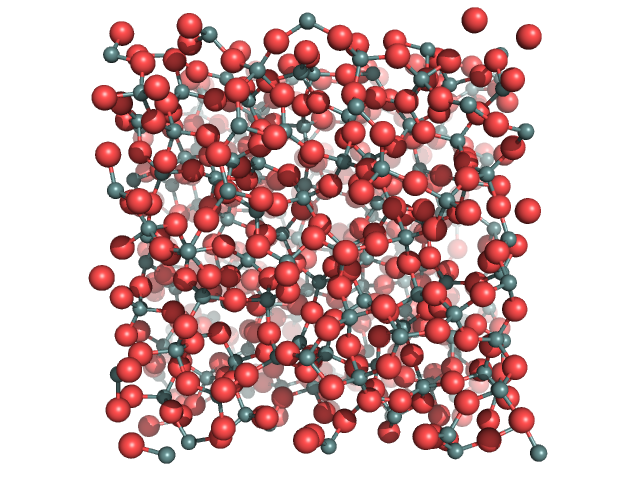
\includegraphics[scale=.25]{GeO2-all.png}
 \label{fig:selectatoms-con}
}
\subfigure[Nuevama configuraci\'on at\'omica en la cu\'al se ha eliminado una regi\'on del espacio.]
{
 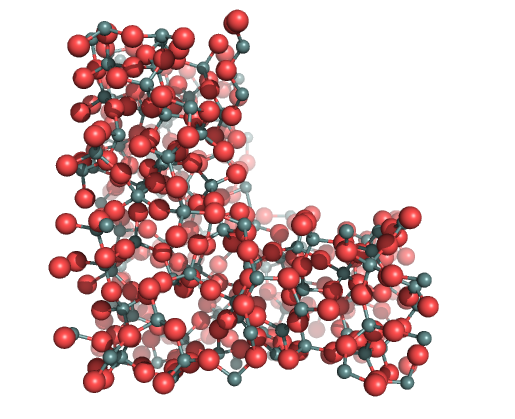
\includegraphics[scale=.30]{GeO2-selat.png}
 \label{fig:selectatoms-sin}
}
\caption{Configuraci\'ones at\'omicas antes y despues de aplicar selectatoms, muy \'util para dise\~nar pel\'iculas con defectos o elementos distintos dentro de una celda, un posterior an\'alisis tambien se puede llevar a cabo por regiones.}
\label{fig:selectatoms}
\end{figure}
